\section{Introduction}

\noindent{\bf Motivation.}
CUDA has become the \textit{de facto} standard for deep learning training because modern frameworks such as PyTorch and TensorFlow are deeply integrated with NVIDIA’s optimized GPU libraries~\citep{nvidia2025cudnn}. 
Efficient CUDA kernels are crucial for accelerating deep learning workloads~\citep{dao2022flashattention,dao2023flashattention2} . 


However, developing high-efficiency CUDA kernels is known to be challenging with a steep learning curve, requiring deep expertise in GPU architectures and parallel programming \citep{onegraph}.
For example, it took more than 2 years from the debut of the Hopper GPU architecture to the release of FlashAttentionV3~\citep{shah2024flashattention3fastaccurateattention}, which is specially designed for Hopper GPUs. 

This high development barrier has driven growing interest in finding automated ways of generating highly efficient and customized CUDA kernels. For example, some work~\citep{DBLP:conf/pldi/TilletKC19}~\citep{chen2019learningoptimizetensorprograms} employs auto-tuning and evolutionary search to automatically explore kernel implementation spaces and optimize low-level parameters for specific hardware. More recently, there has been a growing interest in leveraging large language models (LLMs) to perform such tasks. LLM is believed to hold great promise in generating efficient and high-quality kernels, due to its capability of code generation in other domains, such as Python and C++~\citep{dong2025surveycodegenerationllmbased,jiang2024surveylargelanguagemodels}. 



\noindent{\bf{ Existing Works and Key Challenges.}} Generally, using LLMs for CUDA kernel generation is still in an early stage. In KernelBench~\citep{ouyang2025kernelbenchllmswriteefficient}, the authors attempt to directly use state-of-the-art (SOTA) models, such as OpenAI-o1 and Claude-3.5-Sonnet, to generate kernels. However, it has been observed that these SOTA models still struggle to produce correct or performant kernels out of the box, revealing fundamental limitations of existing LLMs in this domain. 

To address this gap, recent studies have explored two main paradigms. The first approach is based on reinforcement learning (RL)~\citep{schulman2017proximalpolicyoptimizationalgorithms,shao2024deepseekmathpushinglimitsmathematical}. CUDA-L1~\citep{deepreinforce2025cudal1} and Kevin~\citep{kevin-multi-turn-rl} adopt RL to enhance LLMs' ability to generate correct and performant CUDA code. 

The second approach is based on AI agents. In particular, in an independent and contemporaneous work \citep{lange2025robustagenticcudakernel}\footnote{published on arxiv Sept 16th, 2025}, researchers have explored agentic frameworks at inference time. 
Agents project PyTorch methods into CUDA kernel designs, then the CUDA kernels are further refined by sampling new kernels and verification filtering.
This design effectively improves correctness in CUDA kernel generation without the high cost of RL training.


Despite these advances, several key challenges remain:

\noindent \textbf{(C1) Limited kernel efficiency.}  
    While RL-based methods improve LLMs' ability to generate CUDA kernels, their optimization capability remains insufficient.  
    For example, the kernels generated by Kevin-32B only achieve an average speedup of 1.10$\times$ over KernelBench Level 1-2, even after sampling 16 parallel trajectories with 8 refinement turns for each kernel  \citep{kevin-multi-turn-rl}.  
    As another example, CUDA-L1 often fails to directly optimize the CUDA kernels, but produces official implementations of PyTorch \citep{deepreinforce2025cudal1} (see Appendix~\ref{app:cuda-l1} for details). 

    
\noindent \textbf{(C2) High training and inference cost.}  
    RL-based approaches such as \citep{deepreinforce2025cudal1,kevin-multi-turn-rl} require substantial computational resources and long training cycles, making them unsuitable for low-resource or rapid-prototyping settings.  
    In addition,  multi-stage agentic pipeline developed by \citep{lange2025robustagenticcudakernel} incurs high inference costs (about 6 H100 hours and \$5 API cost per kernel), which greatly limits its practical applicability of the approach.


\noindent \textbf{(C3) Lack of hardware feedback.}  
Human experts typically follow an iterative workflow to develop CUDA kernels through testing and refinement.  
They rely on hardware feedback like Nsight Compute (NCU)\footnote{Nsight Compute (NCU) is NVIDIA’s official kernel-level profiler for CUDA programs.} to identify bottlenecks and optimize kernels accordingly~\citep{10946796,cudaguide,w4a8gemm}.  
In contrast, RL-based approaches~\citep{deepreinforce2025cudal1,kevin-multi-turn-rl} train LLMs to directly generate or optimize kernels, but do not leverage hardware feedback at all.  
As a result, they rely on blind exploration during generation, lacking targeted guidance.  
This often leads to suboptimal kernel efficiency, limiting their practical applicability.


These challenges raise a natural question: \textit{Can we design a simple but effective hardware-aware approach that reliably produces efficient CUDA kernels at low cost?} 



\noindent{\bf Our Contributions.} 
To address these challenges, we propose \agentname, {\bf a simple,  effective, and low-cost} multi-agent workflow for CUDA kernel generation and optimization, as shown in Figure~\ref{fig:pipeline}. Our workflow is inspired by the iterative workflow of human experts~\citep{10946796,cudaguide,w4a8gemm}, which contains steps such as developing initial kernels, testing correctness, analyzing hardware feedback, and iterative improvement.


This workflow involves two specialized LLM agents that iteratively generate and optimize CUDA kernels: a Coder, which generates kernels given task instructions and Judge feedback, and a Judge, which analyzes kernels and hardware feedback to guide the Coder generation. One key novelty of \agentname~is its integration of external hardware feedback, including GPU specifications and Nsight Compute (NCU) metrics, enabling the Judge to identify performance bottlenecks like human experts and provide targeted optimization guidance to the Coder.



Compared to single-LLM approaches that  generate and evaluate code using the same LLM, our framework separates these roles into an {\it independent} Coder and Judge, enabling more specialized reasoning and more reliable iterative refinement.
Unlike RL-based methods, \agentname~is  training-free, avoiding the substantial cost of policy training. It is also  hardware-aware, allowing it to tailor CUDA kernel optimizations to the underlying system, making the proposed framework easily generalizable across different GPUs.
Finally, in contrast to existing multi-agent frameworks \citep{lange2025robustagenticcudakernel}, \agentname~is lightweight and cost-efficient, running in just 26.5 minutes on a single RTX 6000 GPU and about \$ 0.3 per kernel in API on average, while still achieving significantly better performance.


We evaluate \agentname~on 250 KernelBench tasks from Level 1 to Level 3. Though these tasks are challenging, \agentname~attains a 97.6\% correctness rate and delivers an average speedup of 1.68× over PyTorch baselines, which significantly outperforms advanced RL model like Kevin-32B, advanced frontier model like OpenAI-o3~\citep{openai2025o3systemcard} and Agentic Baseline~\citep{lange2025robustagenticcudakernel}, shown in Figure~\ref{fig:evolution_path}. Further, we have conducted comprehensive ablation studies of the features of \agentname, such as its effectiveness across multiple GPU architectures, its inference-time scalability by increasing the number of generation, and the effect of different base models. Overall, we observed that the proposed  \agentname~achieves robust performance in all these settings. 


These findings highlight the key contribution of this work: The proposed LLM agent workflow \agentname~is simple but effective: at very low cost, it  develops performant CUDA kernels for many practical tasks, for a variety of GPU architectures and base models. It also exhibits strong test-time scaling capabilities where solution quality can improve substantially while increasing its iteration rounds. These results demonstrate \agentname's strong practical applicability.




\begin{figure}[htbp]
  \centering
  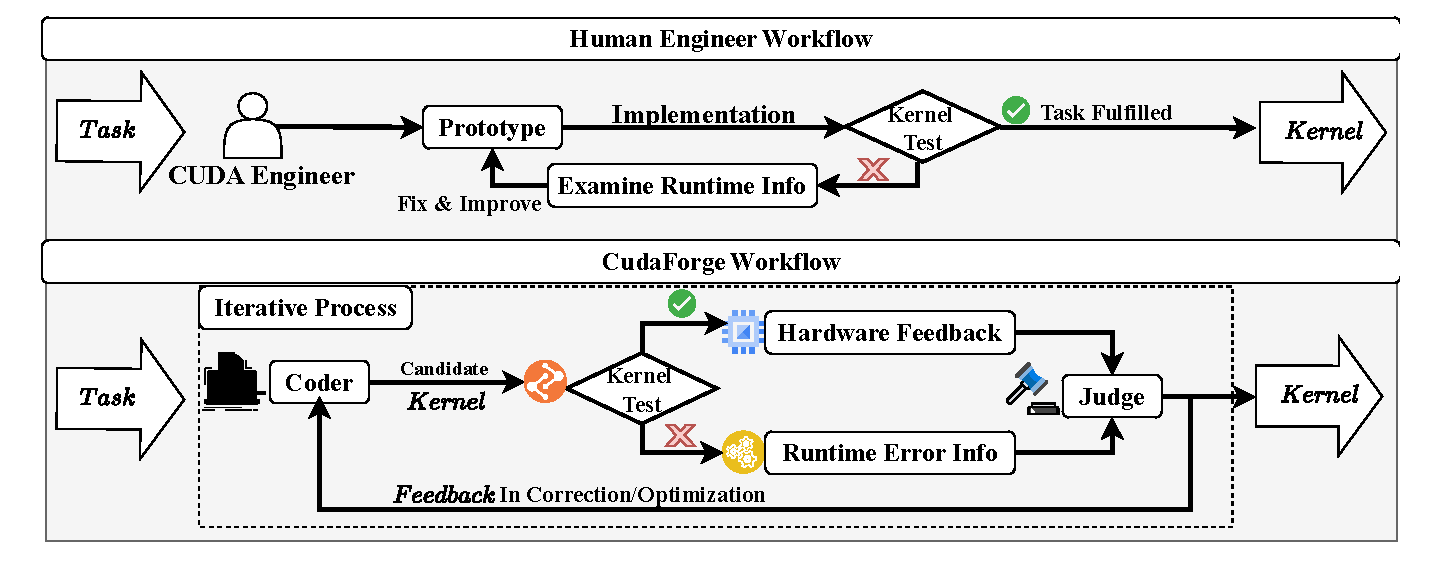
\includegraphics[width=1.0\linewidth]{pic/human_agents_v2.pdf}
  \caption{Comparison between human and \agentname~workflows.
Top: Human experts iteratively refine kernels by writing a prototype, testing it, and analyzing runtime feedback.
Bottom: \agentname~mimics human workflow with two specialized agents (Coder and Judge). The Coder generates candidate kernels, while the Judge analyzes runtime info and hardware feedback to provide correction or optimization feedback. The process iterates until it reaches maximum round $N$.}
  \label{fig:pipeline}
  % \vspace{-8pt}
\end{figure}
